\chapter{\dunyazad/}

\label{ch:dunyazad}

As stated in the introduction, \dunyazad/ has two purposes as a project: first, to produce a \emph{system}, and second, to produce a \emph{theory}.
%
The system is a novel story generator that is focused on generating interesting choices, and on providing fine-grained control over the kinds of choices it uses.
%
The theory is a theory of choice poetics: a theory about how specific choice structures give rise to certain feelings, such as regret.
%
In order to satisfy these two goals, \dunyazad/ uses an answer set solver to turn a logical criteria for a certain kind of choice into an instance of such a choice--this it it's core operating principle.


\dunyazad/'s code therefore largely consists of a set of logical statements describing what a choice structure is and when choices fit into one of several categories.
%
For example, there are statements that define a ``relaxed'' choice.
%
Answer sets for these rules are found using Potassco Labs' \clingo/ solver \cite{Gebser2011}.
%
Besides these rules, there is an external control structure which invokes the solver repeatedly, generating multiple choices and connecting them into a story.
%
The focus of development so far has been on individual choices, but the capacity exists for \dunyazad/ to generate a full branching story.
%
Of course, there is also some imperative code for turning a logical choice structure into English text, in the form of a template-based generation system.
%
The English-generation code and the control code are both written in Python.


The goal of this chapter is to describe in detail how \dunyazad/ functions.
%
First, \cref{sec:dunyazad-asp-and-ctp} describes why \dunyazad/ uses answer set programming in a bit more detail, and how answer set programming (ASP) helps with the theory development goal.
%
\Cref{sec:dunyazad-choice-generation} then describes how \dunyazad/ generates individual choices, while \cref{sec:dunyazad-control} describes the higher-level control mechanism, and \cref{sec:dunyazad-english} describes the template-based English generation component.
%
Finally, \cref{sec:dunyazad-summary} summarizes the entire system and works through an example of how \dunyazad/ generates a choice from beginning to end.

%\section{Goals}

\section{ASP and Critical Technical Practice}
\label{sec:dunyazad-asp-and-ctp}

The idea of critical technical practice started as a call for technical practitioners (and especially AI researchers) to be more aware of the limits placed on their technical approaches by the central metaphors of their fields.
%
In Phil Agre's 1997 \work{Computation and Human Experience} he describes a process of critical examination to identify core metaphors and what those core metaphors marginalize, followed by an inversion that makes those marginalized concepts central \cite{Agre1997}.
%
This process can be used to drive innovation and find hidden limitations in a technical field by scrutinizing it using the tools of critical theory.


Normal AI practice identifies a motivating theory and then attempts to build a system that faithfully operationalizes that theory, taking the theory for granted as an immutable truth.
%
In contrast, critical technical practice seeks to question common assumptions before embarking upon technical projects that use non-standard assumptions, thereby broadening the technical field.
%
\dunyazad/ as a project takes this a step further and sees its driving theory (thoice poetics) as a \emph{product} of technical practice rather than a precursor to it, integrating theory development tightly with system development.
%
\dunyazad/ thus not only actively questions its own theoretical assumptions: it changes them as a matter of course and in fact uses difficulties encountered during technical development to guide these changes.


In order to jointly develop \dunyazad/ as a system and choice poetics as a theory, a special technical approach is required--this is where answer set programming comes in.
%
One could imagine choice-point generators constructed using many different technologies, from case-based reasoning to something as complicated as neural networks.
%
However, most of these would fail to achieve the level of \emph{transparency} required for the system to provide useful feedback to the underlying theory.
%
In a neural-network based approach, for example, it would be very difficult to understand which part of the underlying theory is responsible for a particular generated choice structure, and even more difficult to use experimental results to inform changes in the theory.
%
Answer-set programming as a technical approach is thus motivated by the goal of developing choice poetics along side a technical system for generating choices.


The reason that answer-set programming is useful for critical technical practice is that answer set programs consist of a series of logical statements which dictate which combinations of predicates are allowed in the output.
%
This means that every predicate in the output set can be traced back to a set of rules in the program which allowed it to be present.
%
Sometimes this process is laborious, as many rules may chain together to allow a predicate, but  ultimately, every aspect of an answer-set program's output can be analyzed to figure out which specific statements were responsible for its presence.
%
Furthermore, because those logical statements correspond directly to elements of the underlying theory, the relationship between that theory and the program's output is visible.

% TODO: Better example here?
As an example, \dunyazad/ has rules that define one way in which a choice can be obvious--by having exactly one option which suggests a positive outcome and one or more options all of which suggest negative outcomes.
%
Originally, the criterion that the other options must suggest negative outcomes was not present, but upon looking at generated choices, some clearly didn't fit an intuitive test for obviousness because of their inclusion of neutral options.
%
Identifying the inclusion of these neutral options as the problem was easy, and it was also clear from inspection of the code that without a clause in the definition of ``obvious'' prohibiting neutral options, they would be allowed.
%
The fix at the system level was the extra clause requiring that all options at an obvious choice except the ``correct'' option should suggest negative outcomes.
%
Of course, this was not only a change in the code, it was also a change in the theory, because \dunyazad/'s code is a direct operationalization of choice poetics.
%
Obvious choices don't just have ``only one good option,'' instead they have ``one option which stands out from the rest as significantly better.''


In contrast with many techniques that could be applied to the problem of generating choice points, answer-set programming uniquely enables a tight integration of system development with theory development.
%
The use of answer-set programming as a design choice is thus driven not only by considerations at the system level, but also at the project level: in order for \dunyazad/ to produce both a system and a theory, the use of answer-set programming is critical.
%
In \dunyazad/, answer-set programming supports the aims of critical technical practice by helping make the system's underlying assumptions clearly visible, and by making every change to the system suggest a parallel change to the theory that it implements.

% TODO: Use this mini-rant somewhere?
%In contrast, statistical techniques often hide such assumptions through their use of data which is assumed to be unbiased and universally representative.
%
%In fact, the data sets used to drive statistical artificial intelligence techniques often contain many assumptions, but examination of these is far from straightforward and is seen a peripheral to most technical projects if it is considered at all.


\section{Choice Generation}
\label{sec:dunyazad-choice-generation}

\dunyazad/ generates choices by solving a complicated logic problems.
%
These problems are set up so that any solution will take the form of a choice, and further constraints can dictate certain properties of that choice (for example, that it must be an obvious choice).
%
Broadly, \dunyazad/'s rules can be split into four categories:

\begin{itemize}
\item \textbf{Representational constraints} establish the basic elements that \dunyazad/ arranges to form choices and stories.
\item \textbf{Constituent constraints} define the most basic rules for configuring representative elements to construct choices and stories.
\item \textbf{Aesthetic constraints} carve out a region within the space allowed by the constituent constraints, excluding gibberish and other categorically undesirable configurations.
\item \textbf{Poetic constraints} make distinctions between different desirable configurations and are selectively activated to produce different kinds of choices.
\end{itemize}

To understand how \dunyazad/ functions, it is first necessary to understand \dunyazad/'s (rather limited) view of what a choice is, and how choices fit together to form stories.
%
These things are defined by representational and constituent constraints.


\subsection{Story Representation}


In \dunyazad/, a story is represented as a sequence of actions, each drawn from a pre-determined set.
%
Besides actions, each time point in a story has an initial state, which can include characters, items, and relations between them.
%
This kind of representation is amenable to logical reasoning and similar to representations used in planning-based story generation systems.
%
It is sufficient to represent a wide variety of simple stories focused on action (as opposed to say, character growth or the development of relationships).
%
Luckily, many of the original Choose-Your-Own-Adventure books are focused on actions and consequences, and the format of choice-based narrative lends itself to such stories, because they give rise to interesting choices.


\subsubsection{States}


\dunyazad/'s representational constraints define predicates for ``instances,'' which may be either ``actors'' or ``items,'' as well as ``states'' (binary properties of an instance), ``properties'' (instance properties which can be multi-valued), and ``relations,'' (named directional instance-to-instance links).
%
Besides these things, which can change from one state to the next as a result of the outcomes of actions, instances can have timeless ``surface properties'' like a name, which is stored but cannot be changed by events in the story.
%
\Cref{fig:dunyazad-states} gives examples of each of these and shows how they come together to describe a situation.


\begin{figure}[!t]
\centering
%\includegraphics[width=\textwidth]{fig/dunyazad-states.pdf}
TODO: HERE
\caption[\dunyazad/'s State Predicates]{Predicates used to describe states in \dunyazad/.}
\label{fig:dunyazad-states}
\end{figure}

\begin{figure}[!t]
\centering
%\includegraphics[width=\textwidth]{fig/dunyazad-states.pdf}
\fbox{%
\parbox{\textwidth}{
Scene: \vspace{0.5em}\\
\hspace*{0.8em} ``A merchant carrying some perfume is being threatened by bandits.'' \vspace{0.5em} \\
Representation: \vspace{0.5em} \\
\hspace*{0.8em} \parbox{0.9\textwidth}{ \tt
inst(actor,businessperson\_4). \\
inst(actor,tough\_3). \\
inst(item,treasure\_5). \\
property(type,inst(actor,businessperson\_4),merchant). \\
property(type,inst(actor,tough\_3),bandits). \\
property(type,inst(item,treasure\_5),perfume). \\
relation( \\
\hspace*{0.5em} has\_item, \\
\hspace*{0.5em} inst(actor,businessperson\_4), \\
\hspace*{0.5em} inst(item,treasure\_5) \\
). \\
relation( \\
\hspace*{0.5em} threatening, \\
\hspace*{0.5em} inst(actor,tough\_3), \\
\hspace*{0.5em} inst(actor,businessperson\_4) \\
). \\
surface\_property(name,inst(item,treasure\_5),"perfume"). \\
}
}
}
\caption[\dunyazad/ State Example]{An example scene description using \dunyazad/'s internal representation, showing the most-relevant predicates. In real output, there would be many more ``surface property'' predicates describing things like the name and each instance and whether it is plural or singular. Note that each instance is assigned a unique identifier that ends with a number.}
\label{fig:dunyazad-state-example}
\end{figure}



\subsubsection{Actions}

\subsection{Constituent Constraints}

\subsection{Aesthetic Constraints}

\subsection{Poetic Constraints}

\section{High-Level Control}
\label{sec:dunyazad-control}

\section{English Generation}
\label{sec:dunyazad-english}

\section{Summary}
\label{sec:dunyazad-summary}
